In this section, we are going to solve numerically the time-dependent shallow water model in one spatial dimension. At first, we have solid walls at the boundary and thus the waves should be reflected. We will also linearize this non linear model and compare the solution of the linear problem with that of the non linear one. Finally, we will impose non-reflecting boundary conditions.

The shallow water model is given by :
\begin{align*}
h_t+(hv)_x &= 0\\
(hv)_t + (hv^2+\frac{1}{2}gh^2)_x &= 0\\
\text{on }(x,t)\in [0,L]\times [0,\infty)
\end{align*}

The initial condition is given by :
\begin{align*}
h(x,0) &= H+\epsilon e^{-(x-L/2)^2/w^2}\\
v(x,0) &= 0
\end{align*}

Regarding the boundary condition, we imposed solid walls on $x=0$ and $x=L$. We will see in the next section how that is implemented in practice.

\subsection{Numerical solution}
To solve this problem numerically, we implemented a finite volume scheme using the Lax-Friedrichs method. The matlab code is available at the end of the report.

It is a regular finite volume scheme. However, we needed to impose the solid walls boundary condition. This is done, as explained in Leveque chapter 7, by adding two ghosts cells ($Q_0$ and $Q_{N+1}$) containing each $h$ and $hv$ and saying :
\begin{align*}
h_0 &= h_1\\
h_N &= h_{N+1}\\
v_0 &= -v_1 \implies hv_0 = -hv_1\\
v_N &= -v_{N+1} \implies hv_N = -hv_{N+1}
\end{align*}

This will impose an axial symmetry with respect to the boundary and impose the solid walls condition.

Figure \ref{nonLin} shows the results for four seconds and $\frac{\Delta t}{\Delta x}=0.3$. We can see the initial condition as well as the reflection of the waves of the boundaries. We can also see that when the two waves meets around $t=3$, they loose height. However, there is no numerical dissipation since the total height is conserved (this has been checked!). 

Figure \ref{nonL} shows the same results but in a 2D plot. We can see the waves propagate and colliding. We can also note that the side of the wave that is "in front", meaning on the side where the wave goes, is steeper than the other. This edge becomes also even steeper after the collision. We can recognize here a characteristic of non linear hyperbolic PDE's, where discontinuities can appear.

\begin{figure}
\begin{center}
\includegraphics[scale=0.4]{nonLin.eps}
\caption{Results for the non linear system of PDE}
\label{nonLin}
\end{center}
\end{figure}

\begin{figure}
\begin{center}
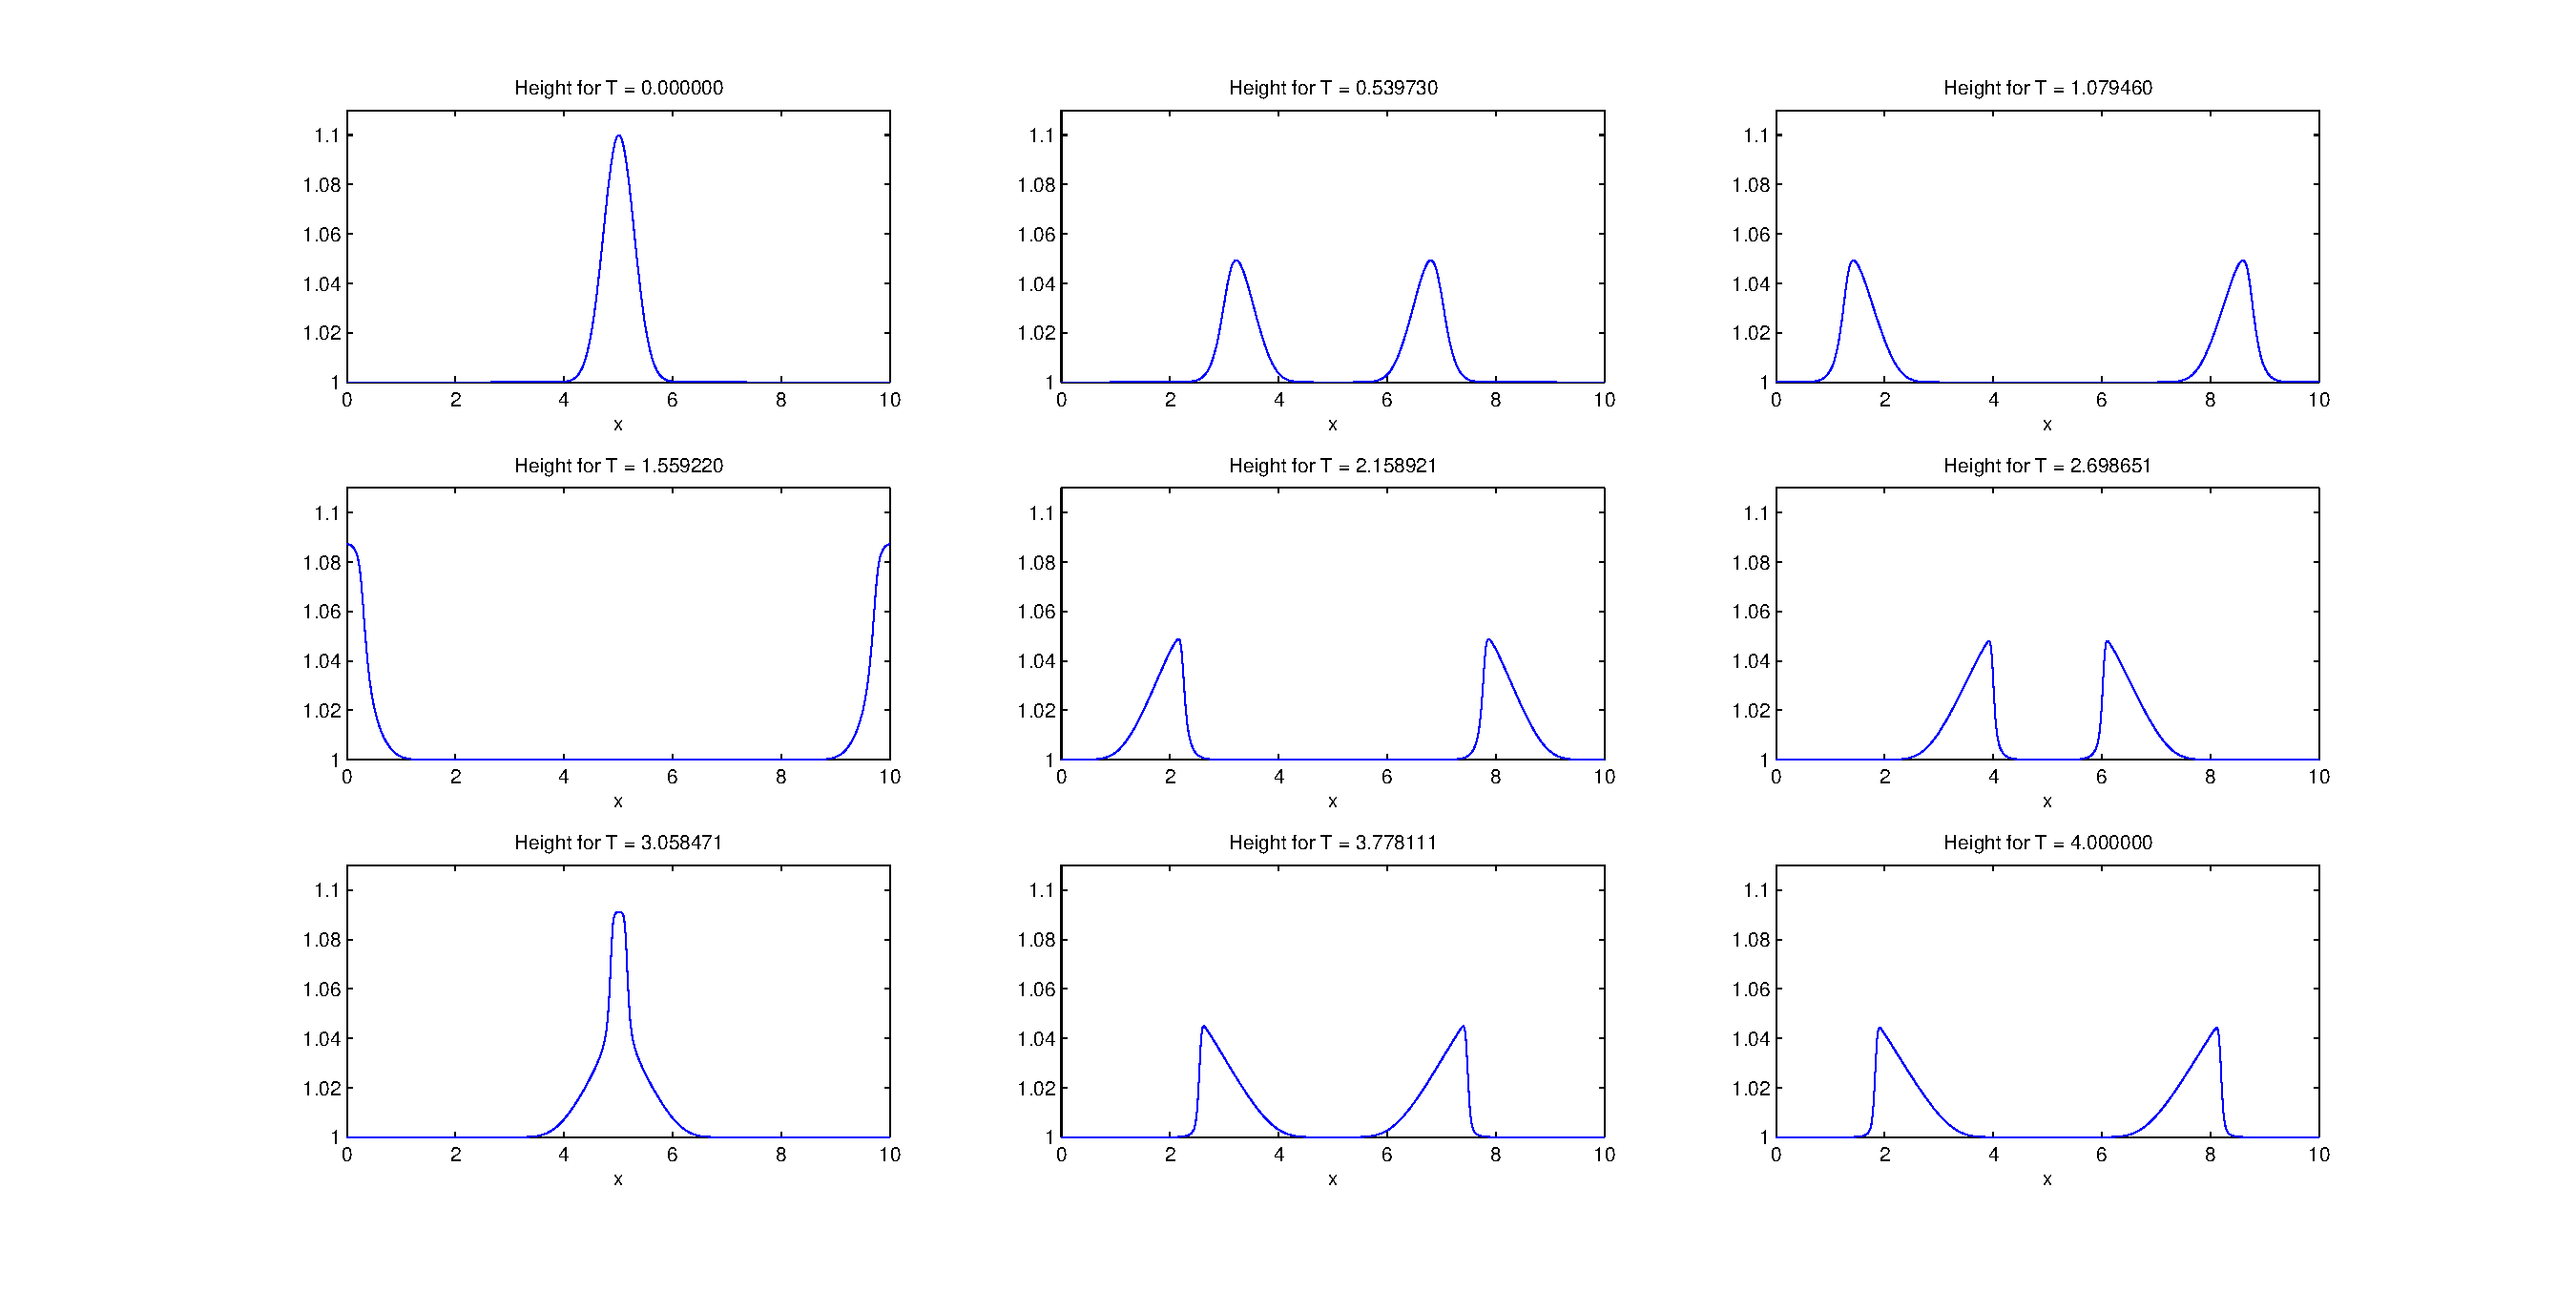
\includegraphics[scale=0.4]{nonL.eps}
\caption{Results for the non linear system of PDE}
\label{nonLin}
\end{center}
\end{figure}


We will now run the program with a larger $\epsilon$. Previously the value was $0.1$, we will now try with $0.4,0.8,1.2$. We can first note that we have to decrease the ratio $\frac{\Delta t}{\Delta x}$ if we increase $\epsilon$. This is because increasing $\epsilon$ also increases the derivative of the height and thus the flux. Thus, to keep a stable numerical scheme, we have to decrease $\alpha$.

Figures \ref{eps04}, \ref{eps08}, \ref{eps12} shows the results for $\epsilon = 0.4,0.8,1.2$ respectively.

\begin{figure}
\begin{center}
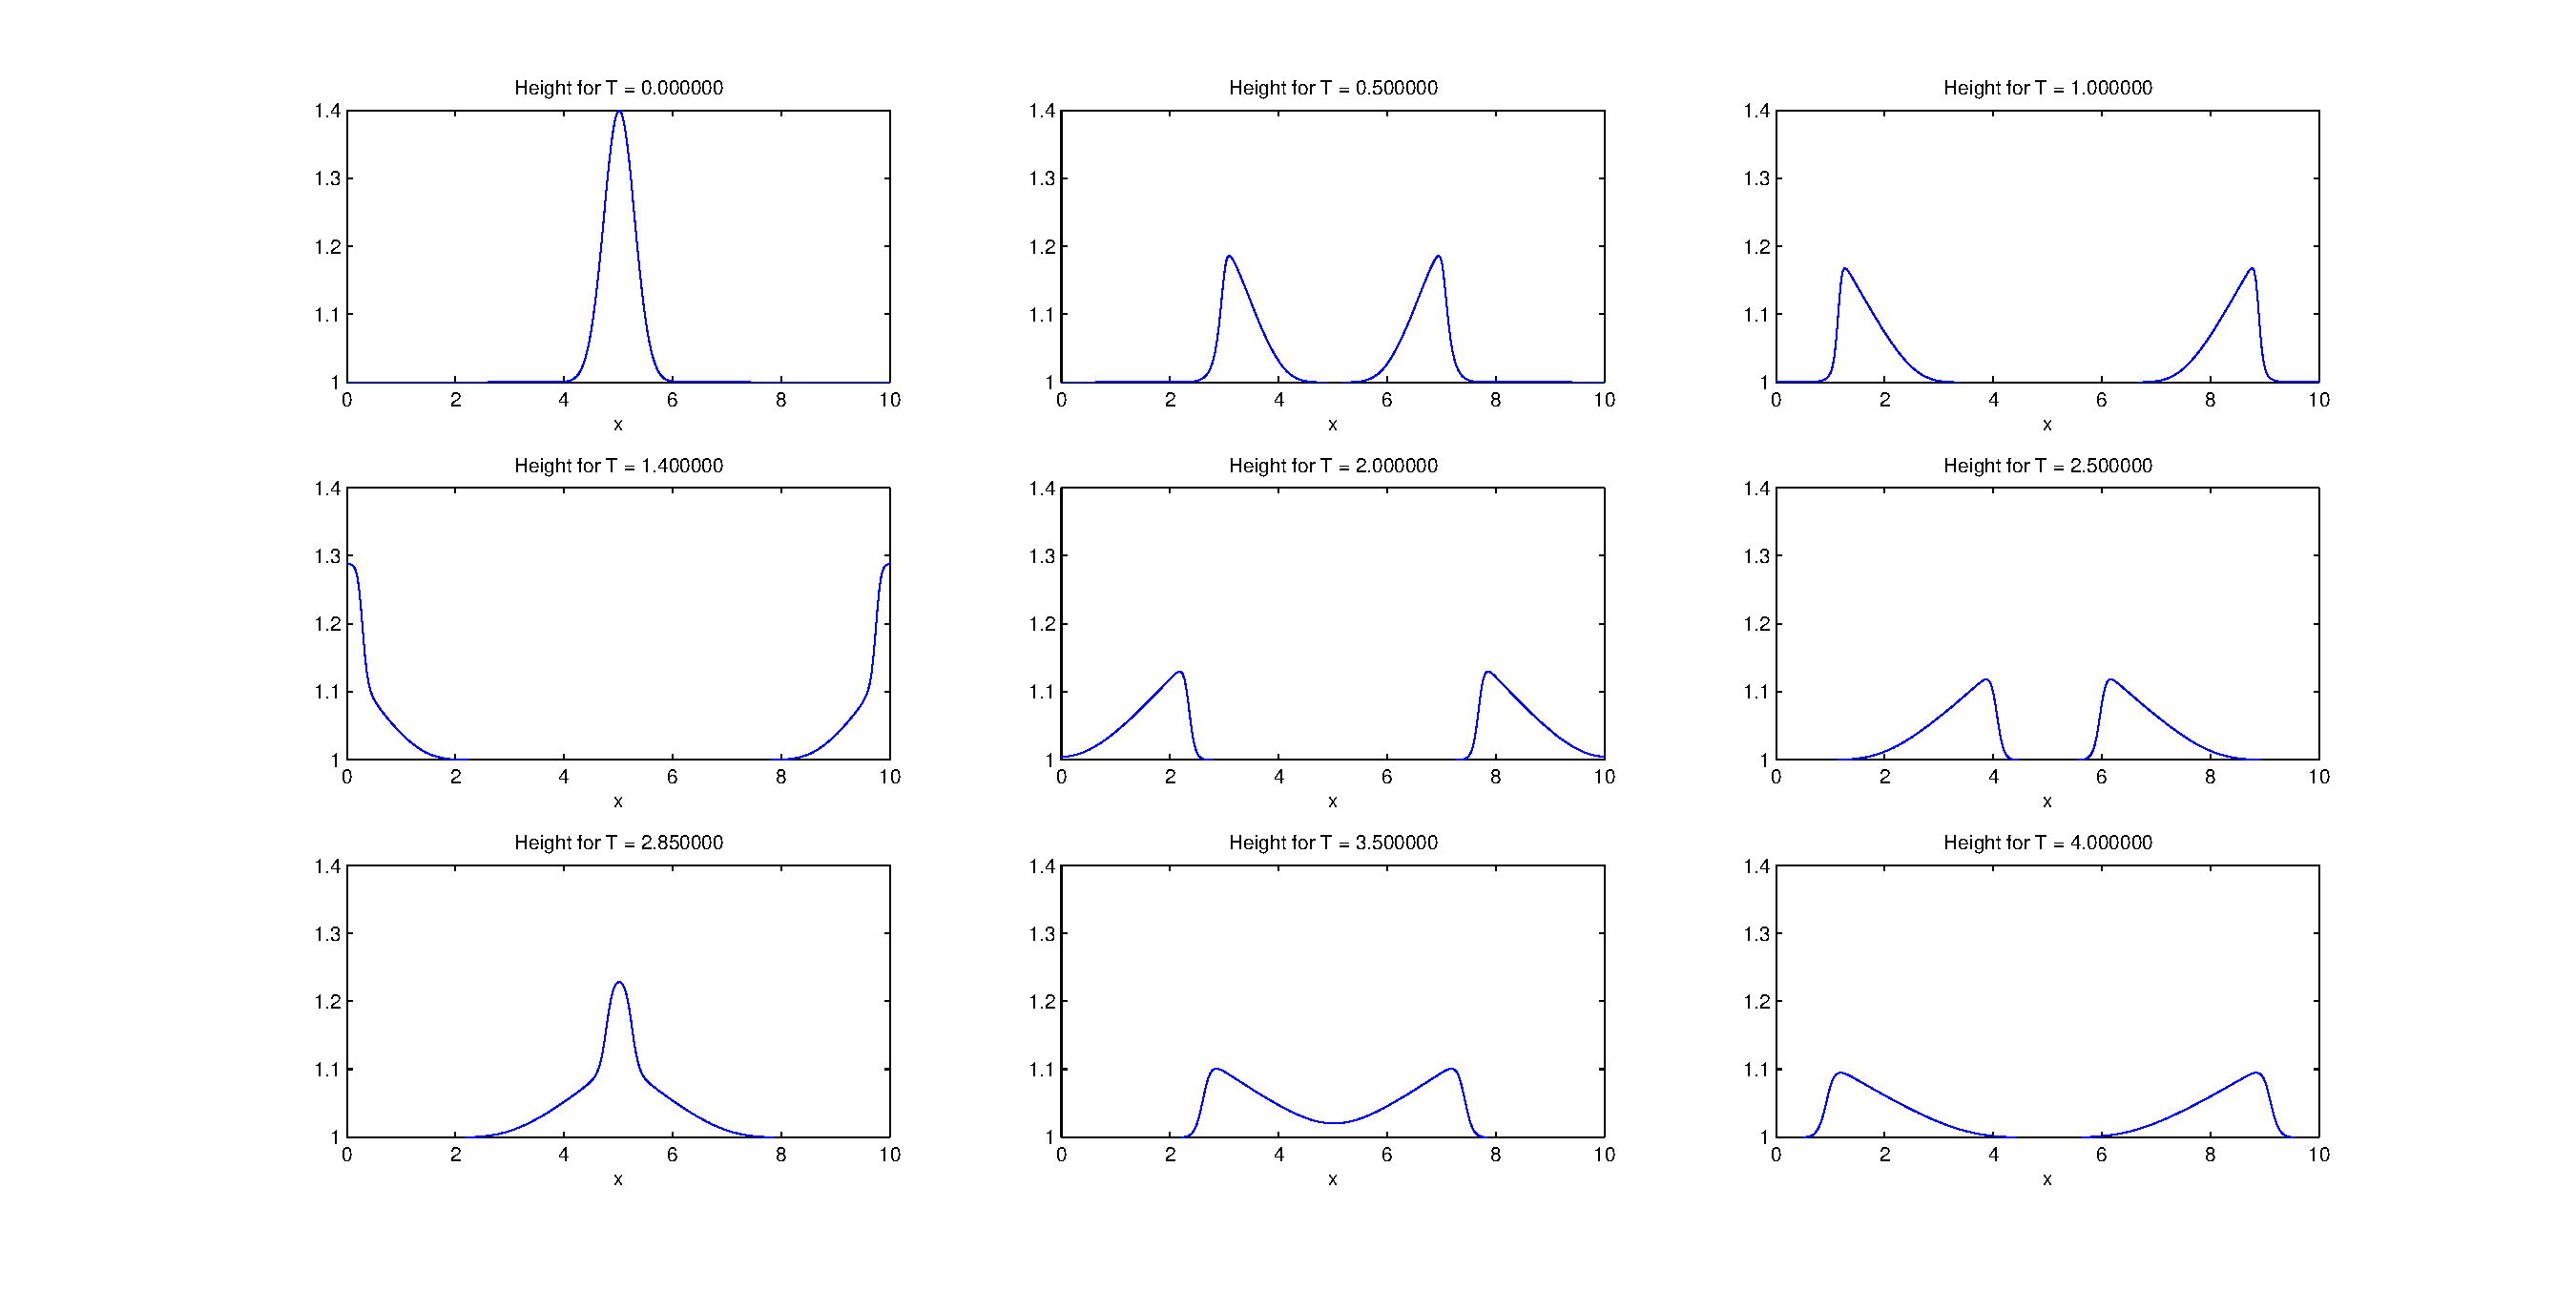
\includegraphics[scale=0.4]{eps04.eps}
\caption{$\epsilon = 0.4$ and $\frac{\Delta t}{\Delta x}=0.25$}
\label{eps04}
\end{center}
\end{figure}

\begin{figure}
\begin{center}
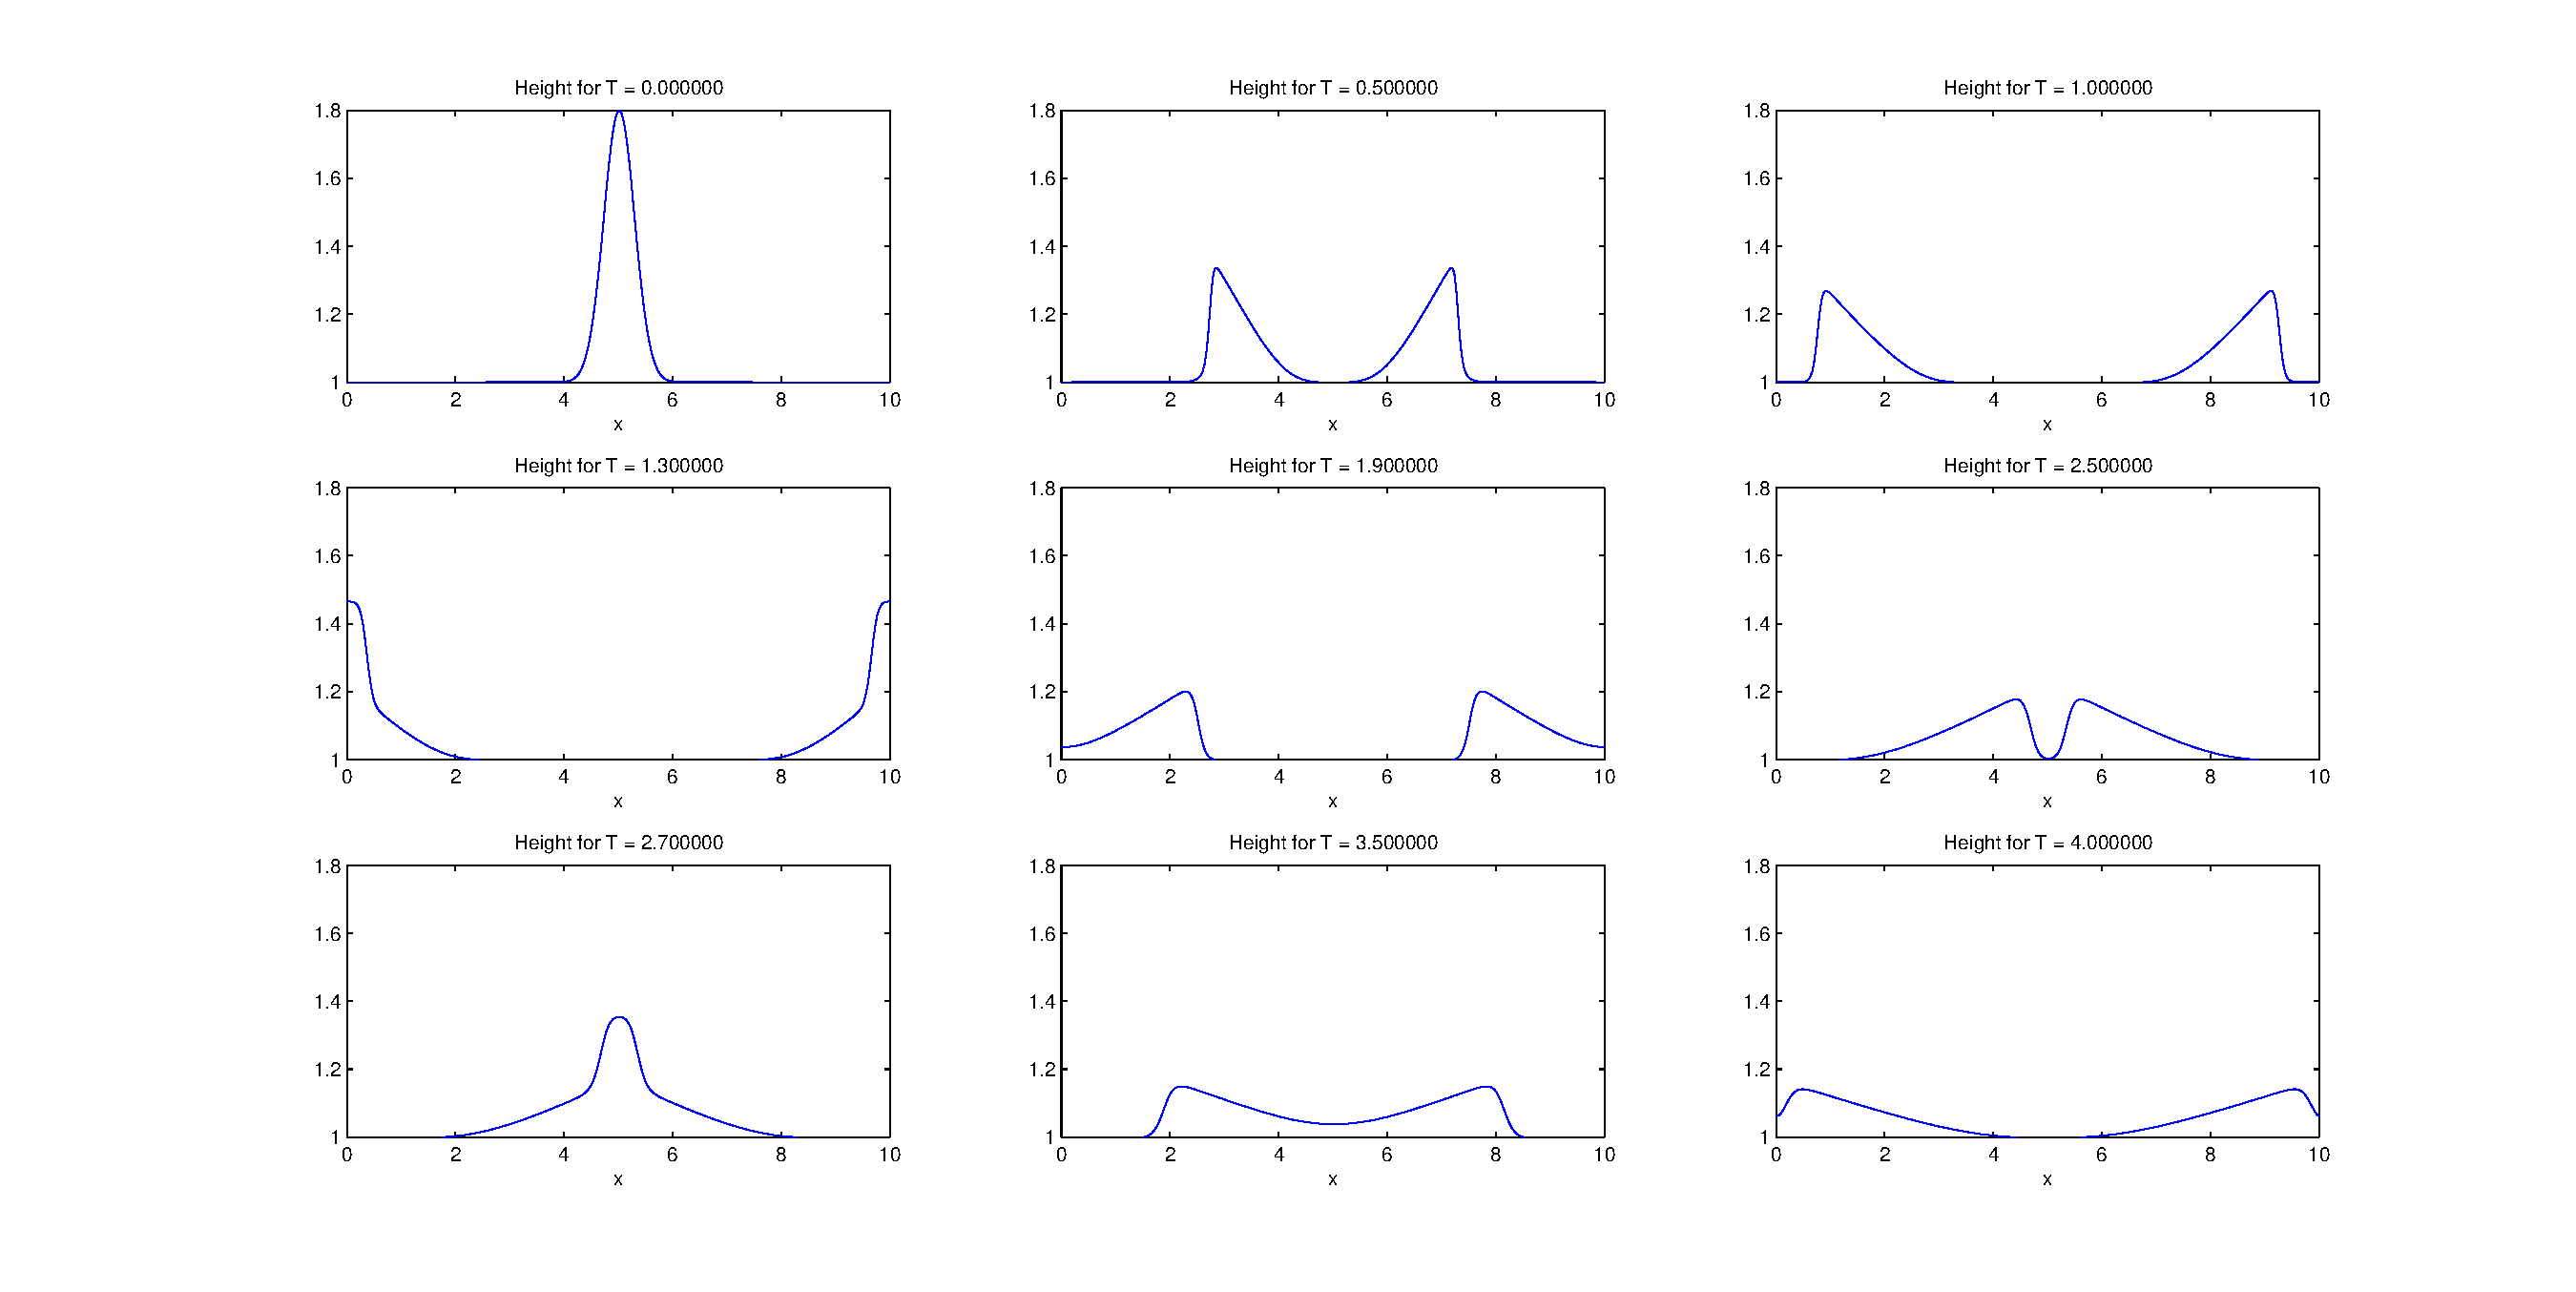
\includegraphics[scale=0.4]{eps08.eps}
\caption{$\epsilon = 0.8$ and $\frac{\Delta t}{\Delta x}=0.21$}
\label{eps08}
\end{center}
\end{figure}

\begin{figure}
\begin{center}
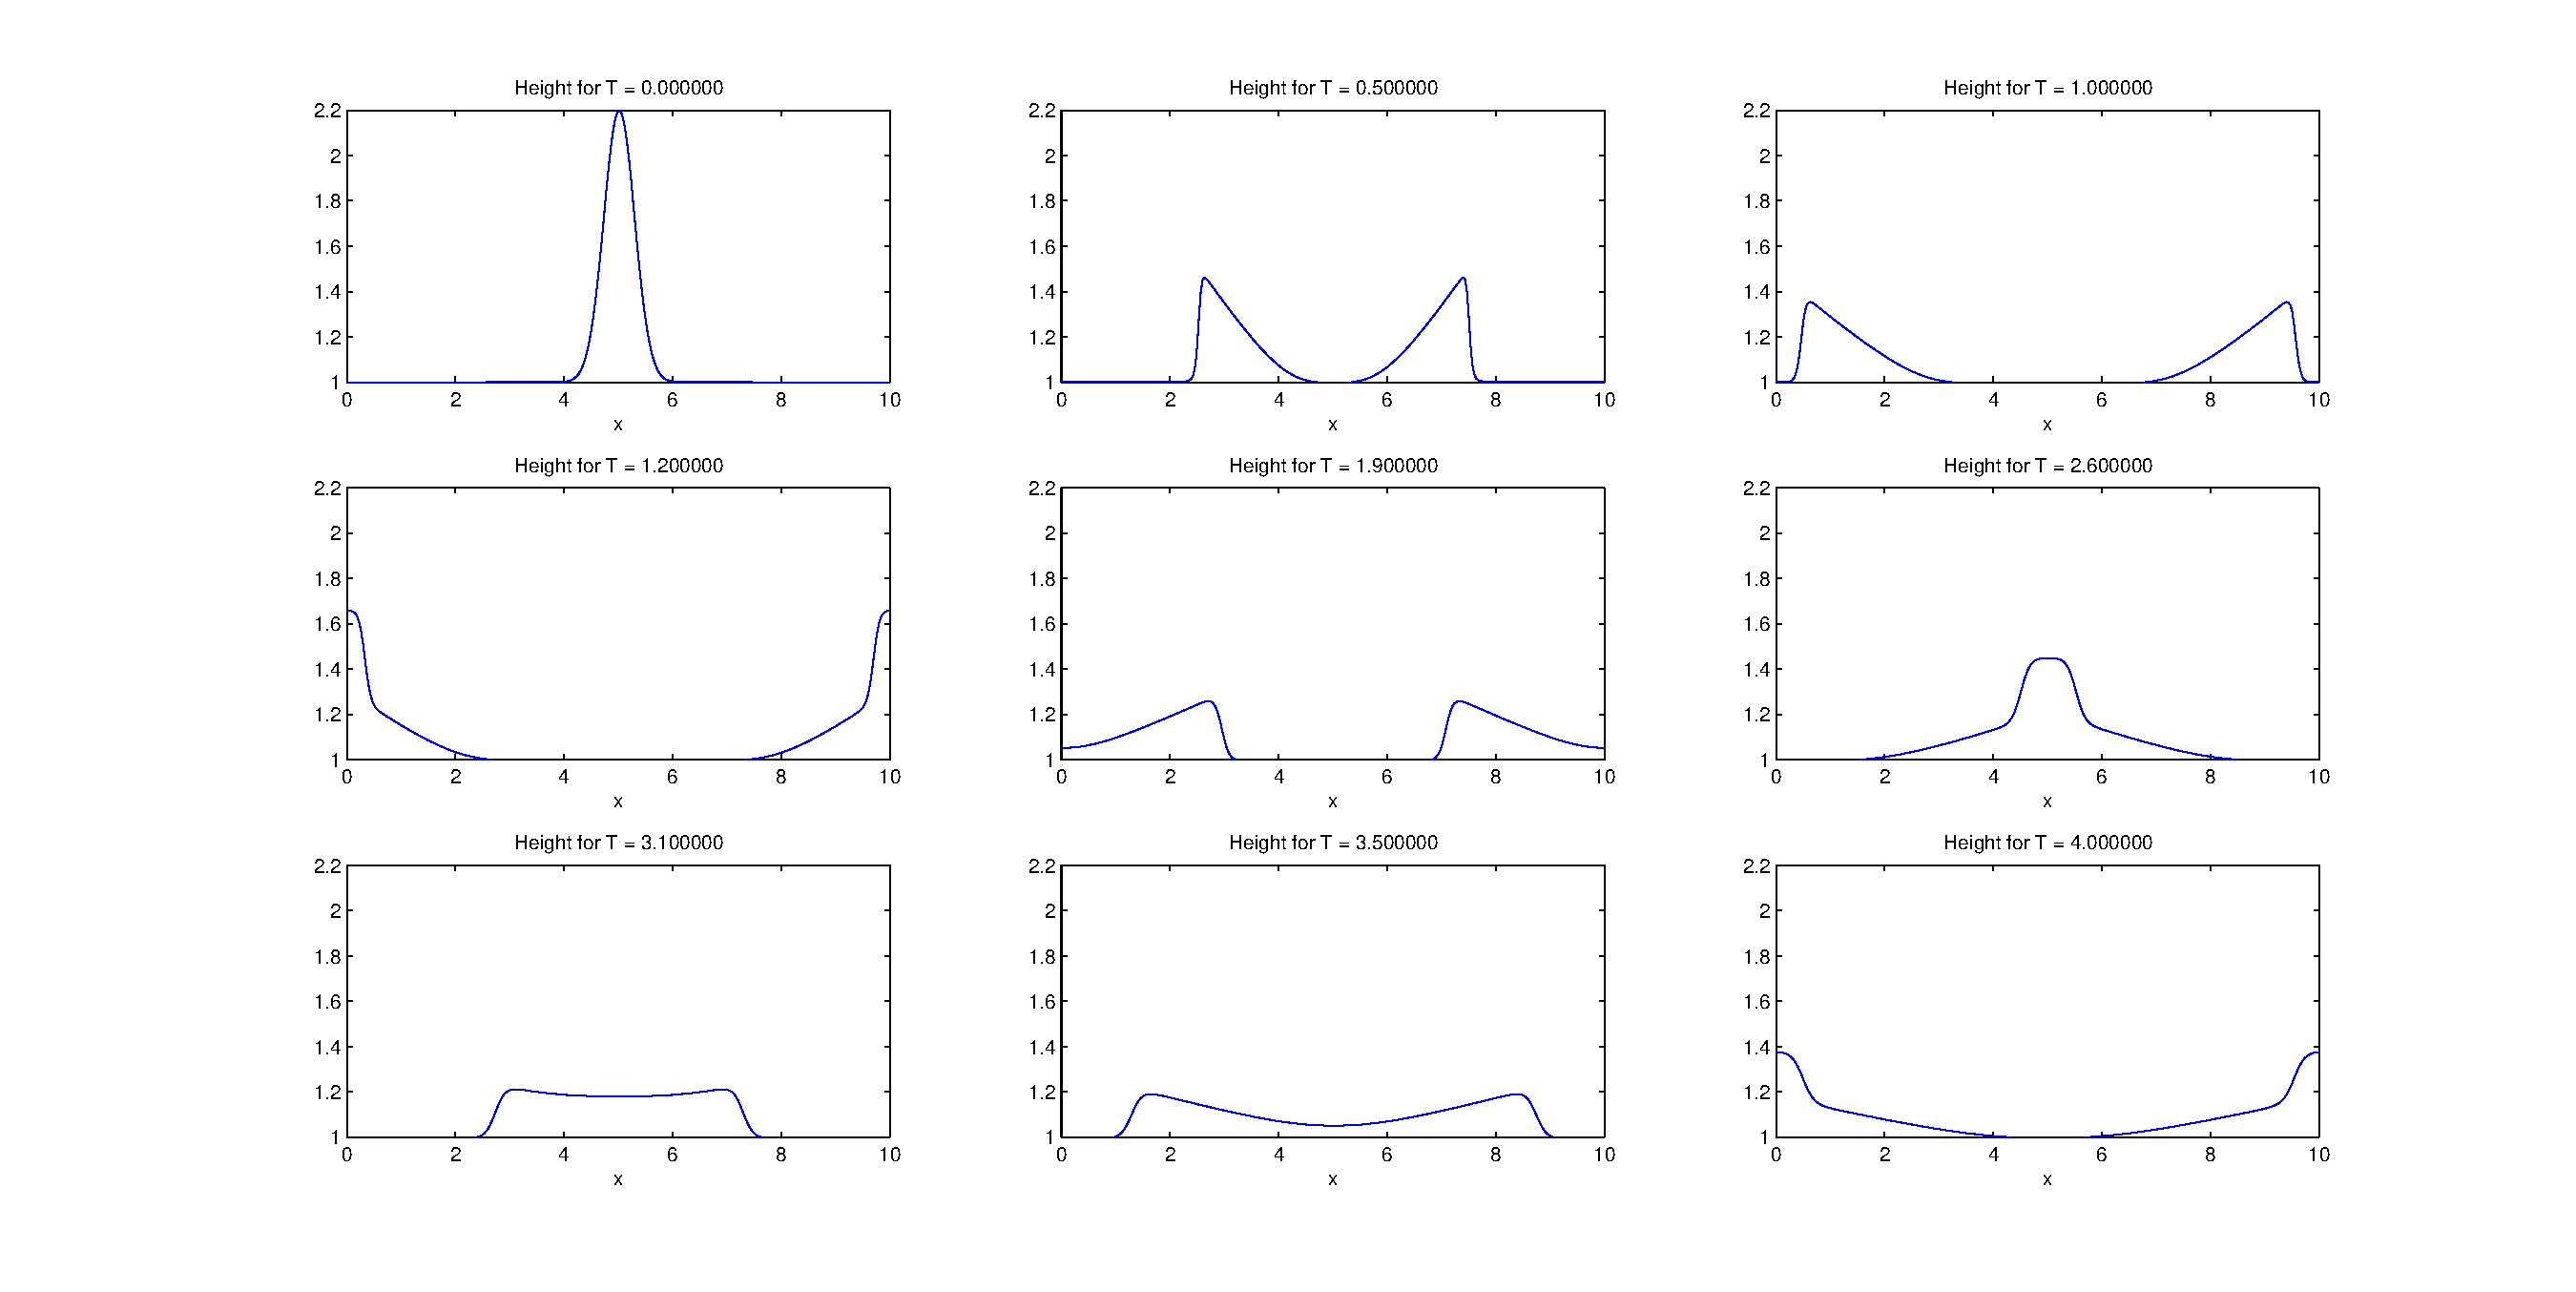
\includegraphics[scale=0.4]{eps12.eps}
\caption{$\epsilon = 1.2$ and $\frac{\Delta t}{\Delta x}=0.19$}
\label{eps12}
\end{center}
\end{figure}

Let us look at the differences between the solutions. There is the amplitude obviously. Because the initial condition is "higher" with a larger $\epsilon$, then so is the height of the propagated wave. We can note, however, that the larger the $\epsilon$ the quicker the wave looses its amplitude. This is intuitive. Indeed, a high thin wave will want to be flatter.

We can also say that the wave speed increases with $\epsilon$. The time needed to reach the boundary is around $1.6$ for $\epsilon=0.1$ but it is $1.3$ for $\epsilon=0.8$ for example. And for the last one, at final time, the waves are already on the other boundary! This is also intuitive that higher waves are quicker.

The collisions look also to affect more the wave. The higher the $\epsilon$, the flatter after each collision the waves look.

Finally, we are going to change the factor $\alpha$ in the numerical scheme. Figure \ref{alpha} shows results after half a second when changing the parameter $C_0$. We kept the ration $\frac{\Delta t}{\Delta x}$ at $0.3$. We can comment that increasing $\alpha$ seems to decrease the amplitude of the wave while making it wider.
\begin{figure}
\begin{center}
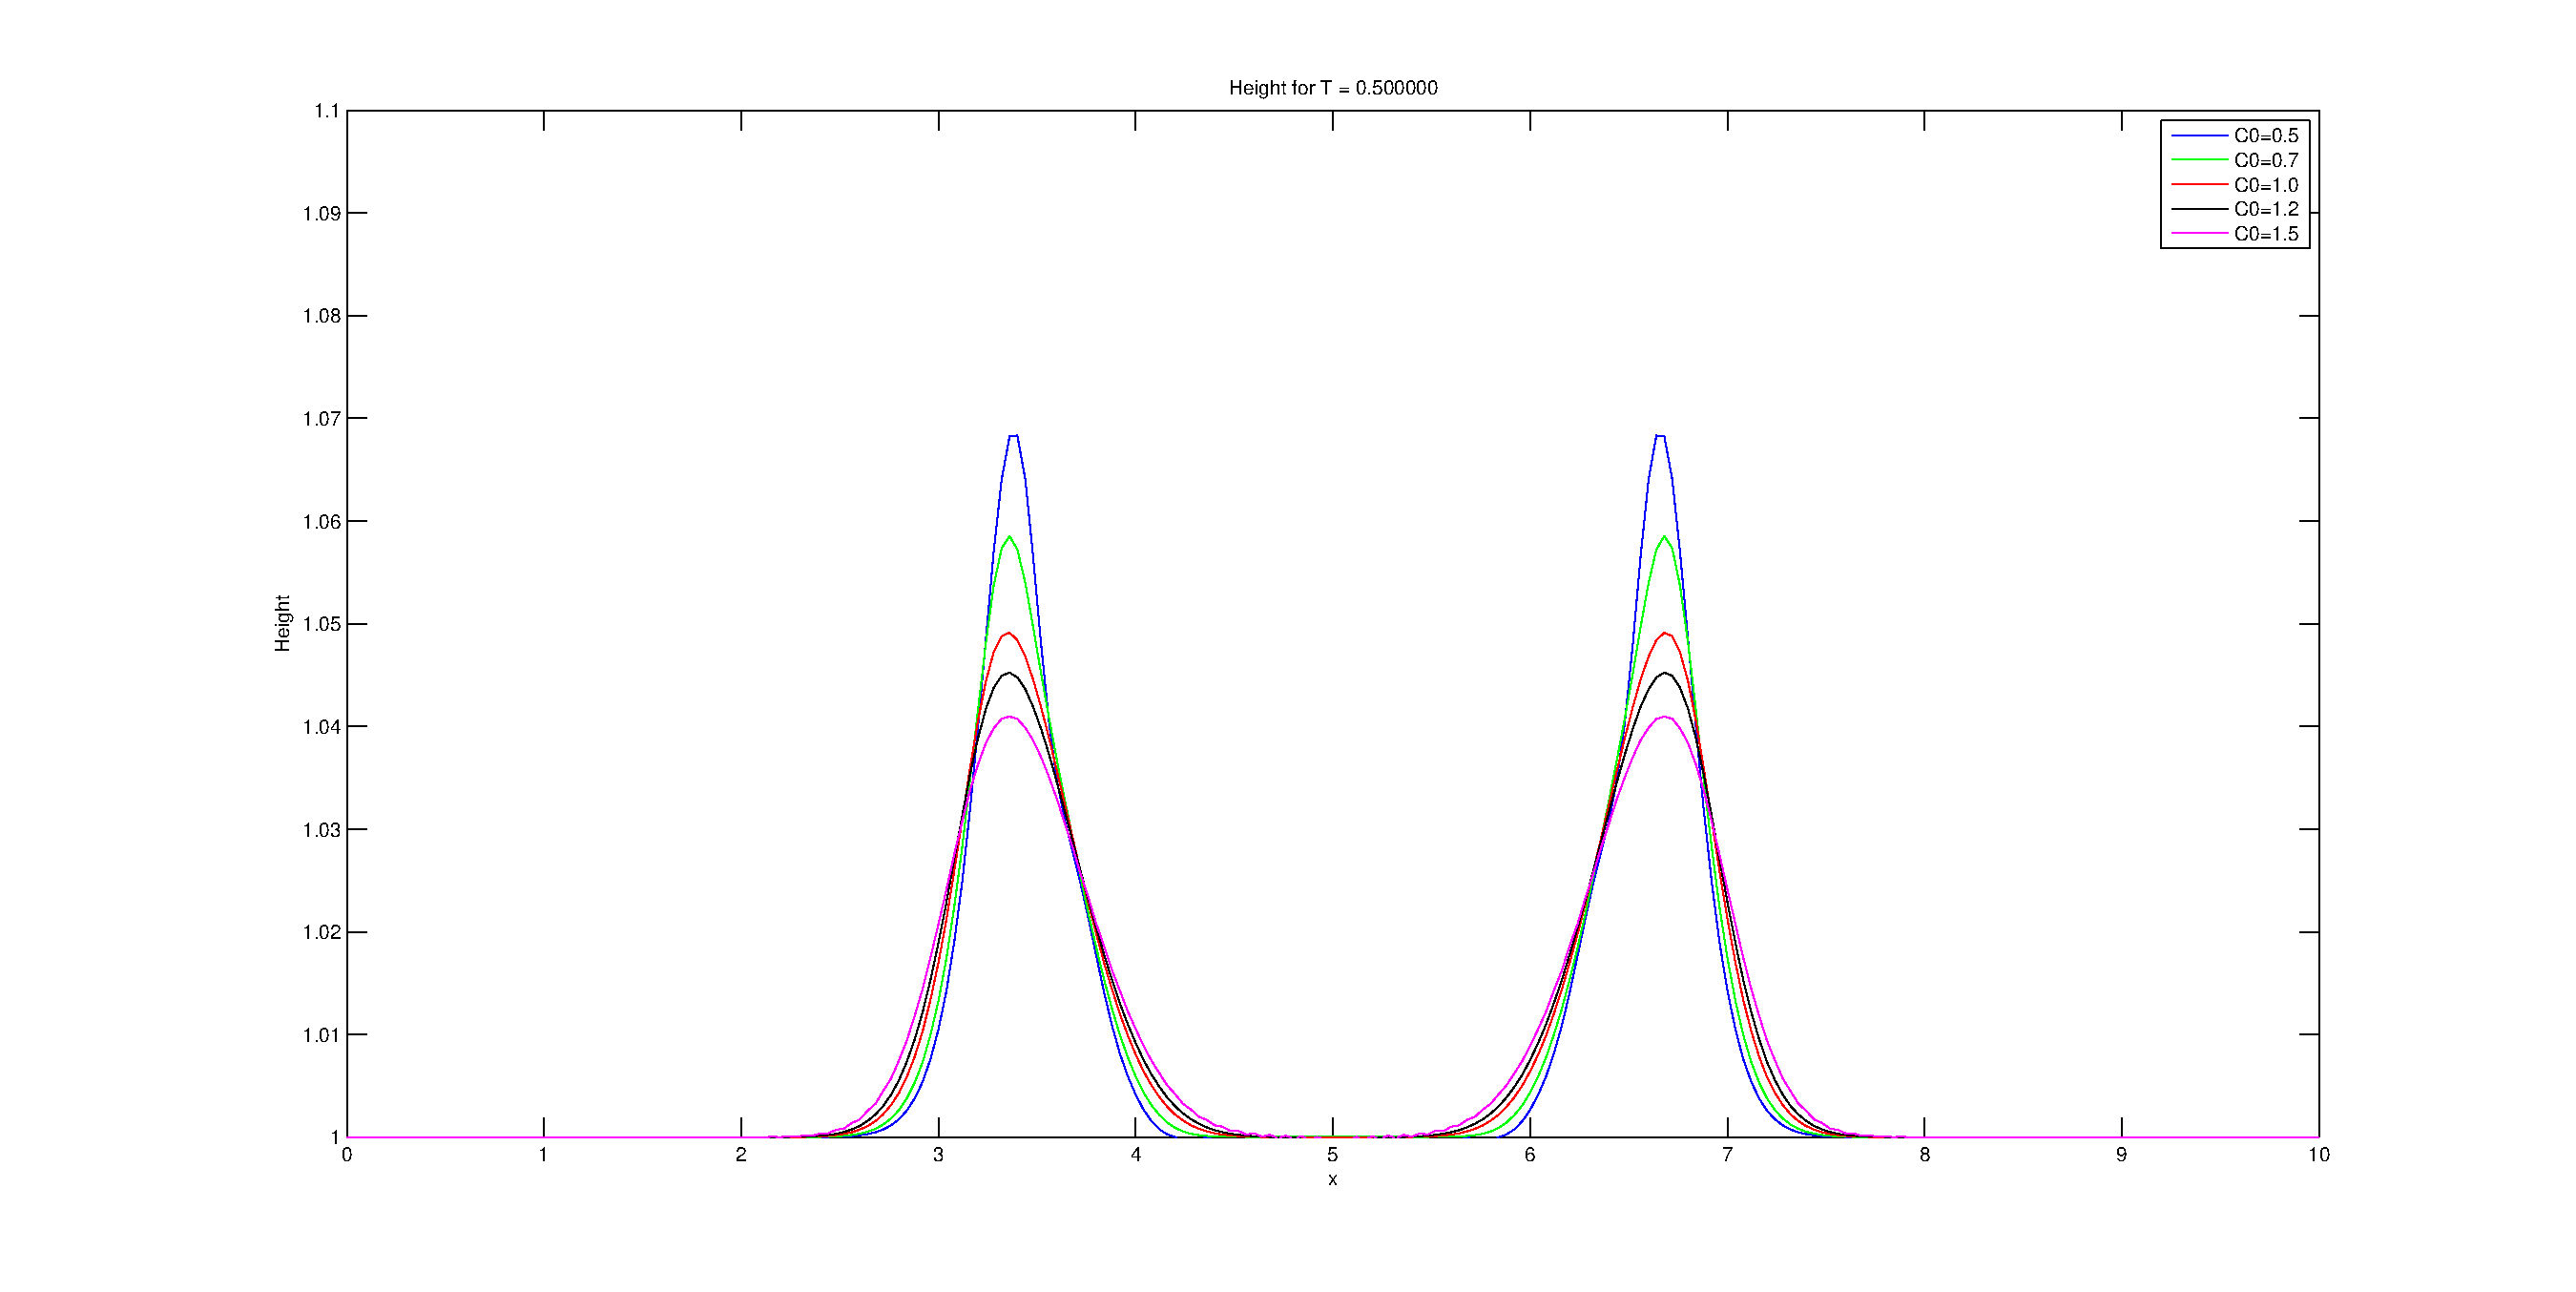
\includegraphics[scale=0.4]{alpha.eps}
\caption{Results when changing $\alpha$}
\label{alpha}
\end{center}
\end{figure}





